% This is part of Un soupçon de mathématique sans être agressif pour autant
% Copyright (c) 2012-2013
%   Laurent Claessens
% See the file fdl-1.3.txt for copying conditions.

\begin{exercice}\label{exoSeconde-0070}

    \begin{multicols}{2}

        À l'aide du graphique ci-contre, donner les solutions (approximatives) des équations
        \begin{enumerate}
            \item
                \( f(x)=1\)
            \item
                \( g(x)=3\)
            \item
                \( f(x)=-2\)
            \item
                $f(x)=g(x)$.
        \end{enumerate}

        À partir du même graphique, répondre aux questions suivantes :
        \begin{enumerate}
            \item
                Est-ce que \( f(1)=3\) ?
            \item
                Combien vaut \( g(3)\) ?
            \item
                Quels sont les points du type \( (2,a)\) à être sur le graphe de \( g\) ?
        \end{enumerate}

        \columnbreak

%The result is on figure \ref{LabelFigExResolutionOSiaMS}.
%\newcommand{\CaptionFigExResolutionOSiaMS}{<+Type your caption here+>}
%\input{Fig_ExResolutionOSiaMS.pstricks}

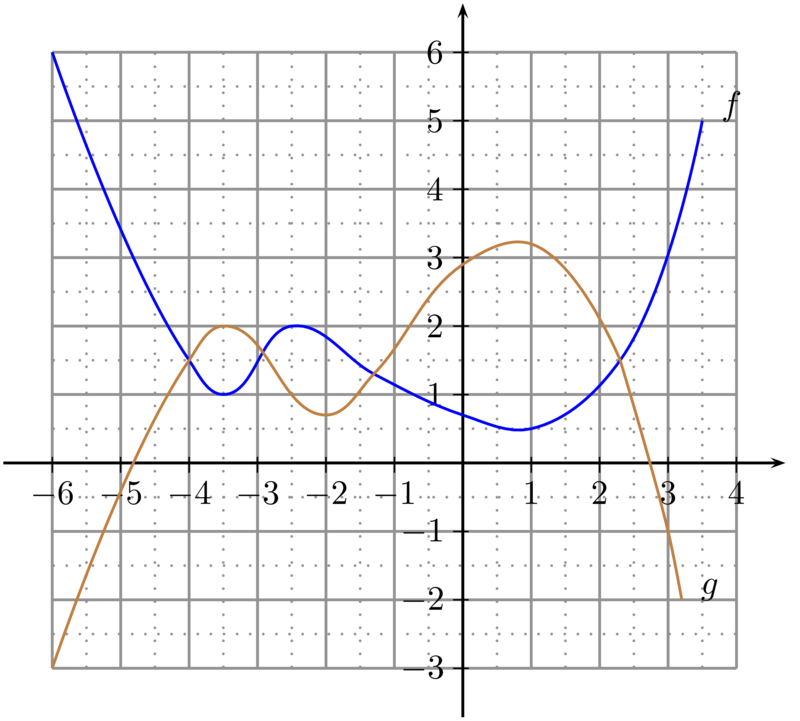
\includegraphics[width=8.0cm]{Picture_FIGLabelFigExResolutionOSiaMSPICTExResolutionOSiaMS-for_eps.png}


    \end{multicols}

\corrref{Seconde-0070}
\end{exercice}
